\documentclass[10pt,a4]{article}
\usepackage[top=0.85in,left=1.75in,footskip=0.75in,marginparwidth=1in]{geometry}

% use Unicode characters - try changing the option if you run into troubles with special characters (e.g. umlauts)
\usepackage[utf8x]{inputenc}
\usepackage{textgreek}
\usepackage[scaled]{helvet}
\usepackage[T1]{fontenc}
\renewcommand\familydefault{\sfdefault}

% file names with period in name, without using braces {}.pdf
\usepackage{grffile}

% clean citationshttps://www.overleaf.com/project/60d45824b01a0838903d992f
%\usepackage{cite}
\usepackage{setspace}
\usepackage{natbib}

\def\cite#1{\hypersetup{citecolor=Teal}\citep{#1}} %changes colour of citep link to Teal.

% clean math
\usepackage{amsfonts}
% \usepackage{amsmath,amssymb,amsfonts}
\usepackage{mathtools}

\usepackage[repeatunits=false,range-units=single]{siunitx}
\newcommand{\micron}{\micro\meter}
\newcommand{\fL}{\femto\liter}
\newcommand{\mmol}{\milli\mol}
\newcommand{\photons}{\micro\mol\per\square\meter\per\second}
\newcommand{\ugml}{\micro\gram\per\milli\liter}
\newcommand{\M}{\textsc{M}}%\mole\per\litre}
\newcommand{\uM}{\micro\textsc{M}}%\mole\per\litre}
\newcommand{\gcdw}{\gram_\text{\tiny DCW}}
\newcommand{\cmol}{\textsc{C$\cdot$}\mol}
\newcommand{\cellvolume}{\milli\liter_\text{\tiny cell}}

\newcommand{\mL}{\milli\liter}
\newcommand{\gpl}{\gram\per\liter}
\newcommand{\mM}{\milli\textsc{M}}%\mole\per\liter}
\newcommand{\ngpul}{\nano\gram\per\micro\liter}

\newcommand{\cuparrow}{\textcolor{blue}{$\pmb\uparrow$}}
\newcommand{\cdoarrow}{\textcolor{red}{$\pmb\downarrow$}}

% nice:
%\usepackage{markdown}

% hyperref makes references clicky. use \url{www.example.com} or \href{www.example.com}{description} to add a clicky url
\usepackage{nameref,hyperref}

% line numbers
\usepackage[right]{lineno}

% improves typesetting in LaTeX
\usepackage{microtype}
\DisableLigatures[f]{encoding = *, family = * }

% text layout - change as needed
%\raggedright
\setlength{\parindent}{0.5cm}
\textwidth 6.25in 
\textheight 8.75in

% Remove % for double line spacing
%\usepackage{setspace} 
%\doublespacing

% use adjustwidth environment to exceed text width (see examples in text)
\usepackage{changepage}

% adjust caption style
\usepackage[aboveskip=1pt,labelfont=bf,labelsep=period,singlelinecheck=off]{caption}

% remove brackets from references
\makeatletter
\renewcommand{\@biblabel}[1]{\quad#1.}
\makeatother

% headrule, footrule and page numbers
\usepackage{lastpage,fancyhdr,graphicx}
\usepackage{epstopdf}
\pagestyle{myheadings}
\pagestyle{fancy}

% no section numbers
\setcounter{secnumdepth}{0}

\fancyhf{}
\rfoot{\thepage/\pageref{LastPage}}
\renewcommand{\footrule}{\hrule height 2pt \vspace{2mm}}
\fancyheadoffset[L]{2.25in}
\fancyfootoffset[L]{2.25in}

% use \textcolor{color}{text} for colored text (e.g. highlight to-do areas)
\usepackage{xcolor}


% this is required to include graphics
\usepackage{graphicx}

% use if you want to put caption to the side of the figure - see example in text
\usepackage{sidecap}

% use for have text wrap around figures
\usepackage{wrapfig}
\usepackage[pscoord]{eso-pic}
\usepackage[fulladjust]{marginnote}
\reversemarginpar

% define custom colors (this one is for figure captions)
\definecolor{Gray}{gray}{.25}
\definecolor{lgold}{RGB}{255, 215, 10}

% MAKROS
\newcommand{\scyst}{\textit{Synechocystis}}
\newcommand{\scst}{\textit{Synechocystis}}

\newcommand{\gene}[1]{\ensuremath{\textit{#1}}}
\newcommand{\gyra}{\gene{gyrA}}
\newcommand{\gyrb}{\gene{gyrB}}
\newcommand{\topa}{\gene{topA}}

\newcommand{\gyrkd}{\ensuremath{\text{gyr}^{\text{KD}}}}
\newcommand{\gyrakd}{\ensuremath{\text{gyrA}^{\text{KD}}}}
\newcommand{\gyrbkd}{\ensuremath{\text{gyrB}^{\text{KD}}}}
\newcommand{\gyrabkd}{\ensuremath{\text{gyrAB}^{\text{KD}}}}
\newcommand{\topakd}{\ensuremath{\text{topA}^{\text{KD}}}}
\newcommand{\topaox}{\ensuremath{\text{topA}^{\text{OX}}}}

\newcommand{\OD}{\ensuremath{\text{OD}_{750}}}
\newcommand{\dOD}{\ensuremath{\text{OD}_{\lambda}}}
\newcommand{\ox}{\ensuremath{\text{O$_2$}}}
\newcommand{\cox}{\ensuremath{\text{CO$_2$}}}

\newcommand{\cqgel}{\ensuremath{C_{\text{gel}}}}
\newcommand{\cqtop}{\ensuremath{C_{\text{relax}}}}
\newcommand{\lk}{\ensuremath{\text{Lk}}}
\newcommand{\lkr}{\ensuremath{\text{Lk}_0}}
\newcommand{\dlk}{\ensuremath{\Delta\text{Lk}}}
\newcommand{\dlkr}{\ensuremath{\Delta\text{Lk}_0}}

\newcommand{\etal}{\textit{et~al.}}
\newcommand{\ie}{\textit{i.e.}}
\newcommand{\eg}{\textit{e.g.}}
\newcommand{\via}{\textit{via}}



% EDITING: rm for publication
\usepackage{todonotes}
\newcommand{\raim}[1]{\begingroup{\color{purple}#1}\endgroup}
\newcommand{\ilka}[1]{\begingroup{\color{blue}#1}\endgroup}
\newcommand{\selma}[1]{\begingroup{\color{red}Salima: #1}\endgroup}
\newcommand{\TODO}[1]{\begingroup\color{red}*** #1 ***\endgroup}

\newcommand{\remove}[1]{\begingroup\color{gray}\endgroup}
\newcommand{\cut}[1]{\begingroup\color{gray}#1\endgroup}


% document begins here
\begin{document}
\sisetup{range-phrase = \text{ - }}


% title goes here:
\begin{flushleft}
{\Large Plasmid supercoiling decreases during the dark phase in
  cyanobacteria: a clarification of the interpretation of
  chloroquine-agarose gels.}

Salima R\"udiger\textsuperscript{1}, 
Anne Rediger\textsuperscript{3},
Adrian K\"olsch\textsuperscript{4},
Dennis Dienst\textsuperscript{1,5},
Ilka M. Axmann\textsuperscript{1},
Rainer Machn\'e\textsuperscript{1,2,*},
\\
\bigskip
\bf{1:} Institut f. Synthetische Mikrobiologie, and\\
\bf{2:} Institut f. Quantitative u. Theoretische Biologie, Heinrich-Heine Universit\"at, Universit\"atsstra\ss{}e 1, D-40225 D\"usseldorf, Germany
\\
\bf{3:} Charit\'e -- Universit\"atsmedizin Berlin, Pressestelle, Charit\'eplatz 1, D-10117 Berlin, Germany
\\
\bf{4:} Physics Department, Freie Universität Berlin, Arnimallee 14, D-14195 Berlin, Germany
\\
%Freie Universität Berlin, Physics Department, Arnimallee 14, 14195 Berlin, Germany
\bf{5:} Photanol B.V, Science Park 406, 1098 XH Amsterdam, The Netherlands
\\
\bigskip
* machne@hhu.de (RM)

\end{flushleft}

\section*{Abstract}
In cyanobacteria DNA supercoiling varies over the diurnal light/dark
cycle and is integrated with temporal programs of transcription and
replication. Woelfe \textit{et al.} (2007, PNAS) have reported that
DNA supercoiling of an endogenous plasmid was progressively higher
during prolonged dark phases in \textit{Synechococcus elongatus} PCC
7942.  This is counterintuitive, since higher levels of negative DNA
supercoiling are commonly associated with exponential growth and high
metabolic flux. Vijayan \textit{et al.} (2009, PNAS) then have
silently reverted the interpretation of plasmid mobility on agarose
gels supplemented with chloroquine diphosphate (CQ), but not further
discussed the differences.
%
Here, we set out to clarify this open issue in cyanobacterial DNA
supercoiling dynamics. We first re-capitulate Keller's band counting
method (1975, PNAS) using CQ instead of ethidium bromide as the
intercalating agent.  A 500x--1000x higher CQ concentration is
required in the DNA relaxation reaction (topoisomerase I) than in the
agarose gel buffer to quench all negative supercoiling of pUC19
extracted from \textit{Escherichia coli}. This is likely due to the
dependence of both, the DNA binding affinity of CQ and the induced DNA
unwinding angle, on the ionic strength of the buffer. Lower levels of
CQ were required to fully relax \textit{in vivo} pUC19 supercoiling
than were used by \citet{Woelfle2007}. Next, we analyzed the
\textit{in vivo} supercoiling of endogenous plasmids of
\remove{\textit{Synechococcus elongatus} and} \textit{Synechocystis sp.}
PCC 6803, at two different CQ concentrations.  This clearly indicated
that negative supercoiling of plasmids does not increase but decreases
in the dark phase, and progressively decreases further in prolonged
darkness.

% now start line numbers
\linenumbers


\section{Introduction}
\textit{In vivo}, the DNA double helix usually exists in a torsionally
strained state, often just denoted as negative DNA supercoiling.  The
energy stored in underwound DNA can be channeled locally at gene
promoters to open and ``read'' DNA in transcription and replication
\cite{Dorman2019}.  In Bacteria, the level of DNA supercoiling is
homeostatically controlled by enzymes but also depends on the
transcription and replication, and in turn influences the
transcription rates of many genes.  In most analyzed bacteria and
conditions, increased negative supercoiling is observed during
exponential growth and decreased during stationary phase or upon
exposure to stress.
%
%The genome-wide levels of DNA supercoiling are difficult to measure,
%and often endogenous or transfected plasmids are used as a proxy
%measurement for \textit{in vivo} supercoiling levels. Plasmids that
%differ topologically (topoisomers) can be separated on agarose gels,
%where each topoisomer forms a distinct band. Plasmids with a higher
%level of negative or positive supercoiling are more compact and
%migrate faster (further) on agarose gels. However, the dynamic range
%of separable topoisomers is small, and the \textit{in vivo} level of
%plasmid supercoiling leads just to broad (smeared) band that consist
%of several topoisomers. Intercalating substances locally unwind DNA
%and thereby can be used to quench supercoiling.  When adding the right
%amount of such an intercalator, e.g. ethidium bromide or chloroquine,
%plasmid supercoiling can be reduced to a level where topoisomers are
%again separable in agarose gels. Increasing the amount of the intercalator
%can further convert originally negatively supercoiled plasmids to
%positively supercoiled plasmids.
%
%Similarly, intercalators can be used together with a supercoil
%relaxing enzyme such as bacterial topoisomerase I to generate a series
%of plasmid samples with continuously less supercoiling. Keller
%combined the use of an intercalator (ethidium bromide) at different
%concentrations in such a relaxation series and on agarose gels. All
%bands from the original state of the plasmid to the fully relaxed form
%can then be counted to determine the so-called linking number deficit
%($\Delta Lk$) of a plasmid sample. $\Delta Lk$ is the difference of the
%number of crossing of the two helix strands aroud each other (the
%linking number) in the supercoiled plasmid and the relaxed form, where
%the helix has about \SIrange{10.4}{10.5}{bp} per helix turn.
%
The DNA supercoiling level of the circular chloroplast genome of the
single-celled algae \textit{Chlamydomonas reinhardtii} showed
fluctuations with the diurnal light/dark cycle \cite{Salvador1998}.
\citet{Mori2001} first suggested that supercoiling could underlie the
regulation of hundreds of genes during the light/dark (diurnal) cycle
in cyanobacteria, the bacterial ancestors of chloroplasts. Indeed,
genome compaction varied over the diurnal cycle in
\textit{Synechococcus elongatus} PCC 7942
\cite{Smith2006}. \citet{Woelfle2007} then used an old method,
separation of plasmid topoisomers by chloroquine-supplemented agarose
gel electrophoresis, to show that the supercoiling level of its
endogenous plasmid varies over the light/dark cycle, and variation
continued in constant light after entrainment to light/dark
cycles. The latter observation is considered a hallmark of the
presence of a circadian clock.  Specifically, they noted a drop in
negative supercoiling of the plasmid already \SI{20}{\minute} after
the transition to light, as well as continuous increase in DNA
supercoiling in prolonged \SI{72}{\hour} darkness. However, a
comparison with a later paper using the same method \cite{Vijayan2009}
shows discrepancies in the interpretation of the agarose gels,
specifically the relative mobilities of more and less supercoiled
plasmid samples.
%
We first review the principles of agarose gel electrophoresis of
plasmids in the presence of DNA intercalators.  To establish the
effect of chloroquine (CQ) on plasmids, we recapitulated Keller's band
counting method but using CQ instead of ethidium bromide (EtBr) as the
intercalating agent, and the pUC19 plasmid isolated from
\textit{Escherichia coli} (\textit{E. coli}) culture in exponential
growth. Next, we extracted endogenous plasmids from the cyanobacterium
\textit{Synechocystis sp.}  PCC 6803 (\scyst{}) grown under light/dark
conditions (\SI{12}{\hour}/\SI{12}{\hour}). Using different CQ
concentrations, we show that, opposite to the interpration by
\citet{Woelfle2007}, negative supercoiling increased (lower $\dlk$)
quickly upon the onset of the light phase and progressivly decreased
(higher $\dlk$) during a prolonged $\SI{48}{\hour}$ dark phase.

\section{Results and Discussion}

\subsection{A Short History of Topoisomer Separation}

The method to measure plasmid supercoiling by agarose gels is the
subject of this contribution and requires some background.  Textbook
plasmid agarose gels show three distinct bands: the ``linear'' form
which underwent a double strand break, likely during extraction; and
the \texttt{oc } (open circular) band, which has only one or more
single strand breaks and thus is still circular. The latter travels
slowest on the gel. And thirdly, intact plasmids travel fastest as a
smeared band, widely known as the \texttt{ccc} band, for the
covalently closed circular form of the plasmid. The band is smeared
since it actually contains several distinct species, denoted
topoisomers, that travel at slightly different speeds in the gel.
%
Topoisomers are identical plasmid molecules (isomers) that differ only
by their level of negative DNA supercoiling, quantified as the
plasmid's linking number (\lk{}) \cite{Crick1976}. The terminology is
from the mathematical field of topology, and \lk{} is the number of
crossings of the two helix strands around each other.  In relaxed
(non-supercoiled) DNA the double helix adopts its minimal free energy
structure with \SIrange{10.4}{10.5}{bp} per helix turn, \eg{} a
circular DNA with \SI{1000}{bp} has $\lkr=\numrange{95}{96}$. Since
this depends on the size of the molecule, levels of DNA superocoiling
are compared as the difference to this relaxed state linking number,
$\dlkr=\lk-\lkr$ and as the supercoiling density
$\sigma=\frac{\dlkr}{\lkr}$.  Negatively supercoiled DNA has $\dlkr<0$
and positively supercoiled DNA has $\dlkr>0$.  Plasmids isolated from
\textit{E. coli} typically have $\sigma=\numrange{-0.08}{-0.06}$,
depending on the growth phase \cite{Liu2018}. Relative topoisomer
abundances follow a Boltzmann distribution around a mean level of
$\sigma$ \cite{Pulleyblank1975, Depew1975, Keller1975b}.

Supercoiled plasmids (\texttt{ccc}) form a more compact molecule than
relaxed plasmids. This is achieved by a higher level structure where
two double helices wind around each other to compensate for the
torsional strain on the double helix. This structure, a so-called
plectoneme, is the origin of the term supercoiling, since it is a
doubly coiled structure: the DNA double helix forms a higher order
``double helix''. The more compact plasmids migrate quicker through
the polymeric meshwork of an agarose gel.
%
If plasmids are artificially relaxed with a nicking-closing enzyme
(NC), such as bacterial topoisomerase I (TopoI), they are still
\texttt{ccc} but now migrate at a speed similar to the \texttt{oc}
form. NC enzymes introduce a single strand break (nick). The torsional
strain in the supercoiled helix leads to rotation of the single
stranded ends. The enzyme then ligates (closes) the ends again and
releases a plasmid with less supercoiling. These reactions will result
in a Boltzmann distribution of plasmids around $\dlkr=0$, with some
positively and some negatively supercoiled \cite{Depew1975}.  These
latter species are already more compact then the relaxed form and they
form distinct bands ``below'' the \texttt{oc} band.


To separate the \textit{in vivo} levels of supercoiling on agarose
gels an intercalating substance can be added to the agarose gel and
the gel buffer.  Intercalating substances reduce the helix rotation
angle between the two bases they bind to, \ie{}, they locally unwind
the helix \cite{Lerman1961, Pritchard1966}. This absorbs some of the
torsional strain of the underwound helix of negatively supercoiled
DNA, and thus reduces the apparent level of supercoiling.  When adding
the right amount of the intercalator, supercoiling is reduced to an
extent which can be separated on the agarose gel.  A similar principle
can be used to generate a series of plasmid topoisomers, starting from
the \textit{in vivo} level of supercoiling and all the way to the
fully relaxed form. The intercalator is simply added to the reaction
mix, supercoiled plasmids are partially relaxed and the NC enzyme can
only remove the remaining level of DNA supercoiling.  After washing
out the intercalator the formerly quenched supercoiling is
re-introduced.  \citet{Keller1975b} developed an elegant method where
different concentrations of the intercalator EtBr are used both in the
NC reaction mix and subsequently on agarose gels to separate
topoisomers. Keller's band counting method allows to simply count all
bands from the original untreated plasmid to the fully relaxed form
across the series of gels, and thereby determine \dlkr{} of circular
DNA isolated from cell cultures.
%
Importantly, the unwinding by the intercalator is not saturated at full
DNA relaxation. Adding more intercalator will result in positively
supercoiled plasmids \cite{Shure1977, Bowater1992}. These are not
affected by typical (ATP-independent) NC enzymes, which only relax
negatively supercoiled plasmids \cite{Wang1971, Kirkegaard1985}. In
contrast, on agarose gels the DNA now changes its migration speed and
positively supercoiled plasmids travel again faster than the relaxed
form. \citet{Shure1977} suggested that with intercalators with lower
affinity the topoisomer separation in agarose gels `\textit{less
  sensitive to variations in experimental conditions}' and first
introduced the use of chloroquine (CQ, all amounts refer to
chloroquine diphosphate) instead of EtBr.

\subsection{Diurnal Plasmid Supercoiling in Cyanobacteria}

\citet{Woelfle2007} used \SI{10}{\ugml} of CQ in their
agarose gel analysis. They state but do not show that they have tested
the relative mobility changes with different CQ levels, and assume
that they are in the range were the plasmids are still negatively
supercoiled.  That is, plasmids that migrated faster on the gel were
interpreted as originally (\textit{in vivo}) more supercoiled (more
negative supercoiling, lower $\lk$). This is reflected in their
gel band annotation and the equation they used to calculate an average
relative mobility ($RM$) of each sample:

\begin{equation}
  RM = \frac{\text{median} - \text{Rel}}{\text{SC} - \text{Rel}}\,,
\end{equation}

where ``Rel'' denotes the migration distance of the upper (slowest
migrating) band, actually the still present \texttt{oc} form.
A lower, fastest migrating band that also appeared in all samples
is denoted as ``SC''. However, it is unclear what this band actually
is, because the supercoiling is quenched by CQ and the actual
supercoiled plasmids travelled as multiple topoisomers. A ``median'' of
their migration speed was used to calculate the $RM$ of each sample.
%
Subsequently, \citet{Vijayan2009} used the same species,
the same endogenous plasmid and the same principle to analyze plasmid
supercoiling after gyrase inhibition and correlate it to global
changes of the transcriptome. They only tested constant light
conditions.  However, they have subtly changed the protocol and used
\SI{15}{\ugml} of CQ in the agarose gels. Without any discussion of
this issue they have further reverted the interpretation of migration
speed to:

\begin{equation}
  RM = 1 - \frac{\text{mean} - \text{oc}}{\text{oc} - \text{rel}}\,,
\end{equation}

where the annotated gels indicate that they inpret the upper, slowest
migrating band as the \texttt{oc} form. They also observe a fast
migrating band in all samples which for unexplained reasons they
denote as a ``rel'' for relaxed. They calculated a ``mean'' migration
distance of the supercoiled topoisomers. The equation likely contains
an error, since $oc-rel$ would be a negative value. Independent of
these unclarities the subtract the $RM$ of Woelfle \etal{} from
1. This implies that they interpret faster migrating topoisomers
as originally less negatively supercoiled. At high intercalator
concentration these should be more positively supercoiled and travel
faster.
%
Choosing more neutral band identifiers makes these
differences clearer:

\begin{align}
  RM &= \frac{\text{target} - \text{upper}}{\text{lower} - \text{upper}}\\
  RM &=1-\frac{\text{target} - \text{upper}}{\lvert \text{upper} - \text{lower} \rvert}\,,
\end{align}

where ``upper'' and ``lower'' refers to their position on the original
gel images, and ``target'' is the mean or median of the topoisomer
distribution.  Despite the opposite meaning of $RM$, both publications
interpret a higher $RM$ as a higher level of negative DNA
supercoiling.
 
This different interpretation of the gels in \citet{Woelfle2007} would
imply that negative supercoiling of plasmids rapidly increases upon
onset of the light phase and would progressively decrease in prolonged
darkness.  \citet{Vijayan2009} measured supercoiling only in constant
light conditions, and did not mention or discuss these discrepancies.
Thus, the DNA supercoiling dynamics within the natural light/dark
cycle of cyanobacteria remains unclear.

\begin{figure}[ht!]
    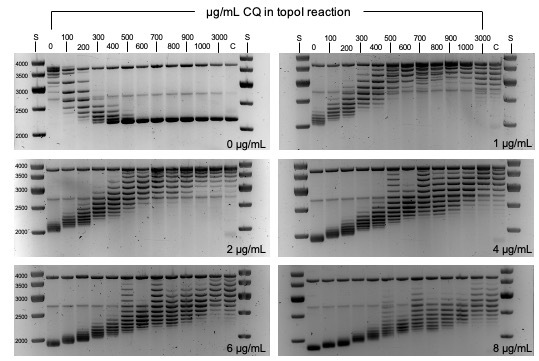
\includegraphics[width=\textwidth]{figures/keller_puc19.jpg}
  \caption{\textbf{pUC19 on 1.2 \% agarose gel supplemented with 0--8
      \si{\ugml} CQ.} Samples of the pUC19 plasmid, isolated from
    \textit{E. coli}, were treated with 0--3000 \si{\ugml} CQ and
    topoI as indicated (lanes). The sample “C” is untreated pUC19 as
    control. Size marker "S" is the GeneRuler 1 kb DNA Ladder. The
    samples analyzed on 6 agarose gels, each supplemented with a CQ
    concentration from 0 to 8 \si{\ugml} as indicated (lower
    right). The top band in each gel is the open circular form. The
    band between 2.5 kb and 3 kb is the linear form of the plasmid.}
  \label{fig:keller} 
\end{figure}


\subsection{Keller's Band Counting Method with Chloroquine and pUC19.}
%
\cite{Keller1975b} analyzed the linking number of the circular genome
of the simian virus 40 (SV40, \SI{5.2}{kb}), propagated in and
isolated from African green monkey cells (CV-1). For this, the DNA was
subjected to \textit{in vitro} relaxation with an NC enzyme
purified from human tissue culture cells (KB-3).  \remove{EtBr concentrations
in the relaxation reaction \remove{(10 mM Tris-HCl, 0.2 M NaCl, 0.05 mM
dithiothreitol, 0.5 \% glycerol, 0.2 mM Na$_2$-EDTA) \todo{re-check
  buffers}} were $\cqtop{}=\SIrange{0}{6.9}{\uM}$.}
%keller fig 1/3: lanes 11 and 9 have in vivo supercoiling
%
Full relaxation of the SV40 DNA in the gel buffer \remove{(40 mM
  Tris-HCl (pH 7.9), 5 mM sodium acetate, 1 mM Na$_2$-EDTA, with
  buffer re-circulation)} was achieved at $\cqgel=\SI{0.06}{\ugml}$,
or with \SI{394.3}{\gram\per\mol},
$\cqgel=\SI{0.15}{\uM}$\remove{0.06/394.3 = 0.00015 umol/ml= mMol =
  0.15 uM}. In the topo I reaction $\cqtop\approx\SI{4.5}{\uM}$ (lane
9 in Figures 1 and 3 of \cite{Keller1975b}) were required to fully
relax the DNA. The \textit{in vivo} supercoiling level of the SV40 DNA
was $\dlkr\approx24$ and $\sigma\approx0.05$.

Here, we propagated the pUC19 vector plasmid (\SI{2686}{bp}) in in
\textit{Escherichia coli} and harvested plasmid in exponential phase
on LB medium. A plasmid relaxation series was performed with the
bacterial NC enzyme TopoI obtained from New England Biolabs. To find
the appropriate CQ concentrations to reproduce Keller's band
counting method, we first analyzed the EtBr concentrations used in the
original publication, considered the ca. 1000x lower binding affinity
of CQ, and adjusted concentrations from there.
%
Figure \ref{fig:keller} shows that the lowest CQ concentration in the
gel ($\cqgel=\SI{1}{\ugml}$) was sufficient to detect a clear change
in the migration of all pUC19 topoisomers. Fully relaxed plasmids
($\cqtop=\SIrange{0}{200}{\ugml}$) had already shifted to positive
supercoiling and migrated faster than without CQ.  Topoisomers treated
with $\cqtop=\SIrange{800}{1000}{\ugml}$ were all close to full
relaxation at $\cqgel=\SI{1}{\ugml}$. The untreated \textit{in vivo}
sample (``C'') appeared fully relaxed at $\cqgel=\SI{2}{\ugml}$, and
shifted to positive supercoiling at $\cqgel>\SI{4}{\ugml}$.  The
topoisomers relaxed at the highest concentration
($\cqtop=\SI{3000}{\ugml}$) appeared with band patterns almost
identical to the untreated control in all gels.  With a molecular
weight of \SI{515.86}{\gram\per\mol} (chloroquine diphosphate),
fully relaxing concentrations of CQ were thus
$\cqgel\sim\SI{3.9}{\uM}$\remove{2/515.86=0.0039 umol/ml = mMol =
  3.9 uMol} and $\cqtop\sim\SI{5.8}{\mM}$\remove{3000/515.86 = 5.8
  umol/ml = 5.8 mMol}.
%
%Thus, the concentration to fully relax the original level of DNA
%supercoiling was \SIrange{1}{4}{\ugml} in the agarose gel buffer (0.5x
%TBE), and \SIrange{1000}{3000}{\ugml} in the CutSmart reaction buffer
%(see Methods for composition).
%
Counting topoisomers across gels, our gels show that the untreated
control has a $\dlkr=\numrange{-15}{-16}$. With \SI{2686}{bp} length,
$\lkr\approx257$ and thus $\sigma\approx0.06$, as expected
for a plasmmid isolated from \textit{E. coli}.

%\paragraph{Discussion: CQ vs EtBr.}
In summary, the intercalator concentrations required to fully quench
the original level of supercoiling of SV40 and pUC19 were $\approx$30x
and $\approx$1000x higher in the reaction buffers than in the gels,
respectively. The CQ concentrations were \numrange{100}{1000}x higher
than the EtBr concentrations in \citet{Keller1975b}.
%
EtBr binds to DNA with relatively high affinity, \eg{}
$K_a=\SI{1.5e5}{\per\Molar}$ in \SI{0.2}{\Molar} Na$^+$
\cite{Gaugain1978}, and each intercalated molecule unwinds the helix
by \SIrange{26}{28}{\degree} \cite{Keller1975b}. CQ has a
lower affinity to DNA, depending on ionic strength of the buffer,
\eg{} $K_a=\SI{3.7e4}{\per\Molar}$ in a \SI{50}{\mM} phosphate buffer
and $K_a=\SI{3.8e2}{\per\Molar}$ with \SI{0.1}{\Molar} NaCl
\cite{KwakyeBerko1989}. The DNA unwinding angle induced by CQ is lower
and, unlike EtBr, also depends on the ionic strength of the buffer,
with a maximum of \SI{17}{\degree} at \SI{0.05}{\M} salt concentration
\cite{Jones1980}.  Additionally, intercalator effects on DNA
supercoiling as well as supercoiling-dependent conformations
of circular DNA could be sequence dependent \cite{Vetcher2010}.
%
Together these factors likely explain the differences in
concentrations required for full relaxation of SV40 by EtBr, of pUC19
by CQ, and between the gel and reaction buffers in both
implementations of Keller's band counting method.

%The \dlk{} of circular DNA itself affected by the ionic conditions and
%potentially DNA sequence \cite{Vetcher2010}



\begin{figure}[ht!]
  \begin{minipage}{.49\textwidth}
    
\includegraphics[width=\textwidth]{figures/diurnal/20130620_pCA_CQ1.png}
    
    \vspace{-.5cm}
    \textbf{A}
    
    
\includegraphics[width=\textwidth]{figures/diurnal/20130821_pCA_CQ20.png}
  \end{minipage}
  \begin{minipage}{.39\textwidth}
    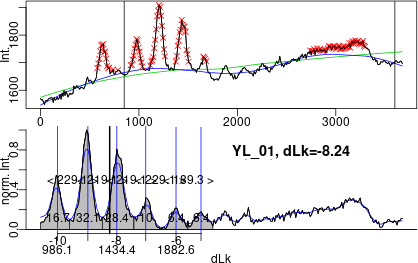
\includegraphics[width=\textwidth]{figures/diurnal/YL_01_cropped.png}
   
    \vspace{-.5cm}
    \textbf{C}
    
    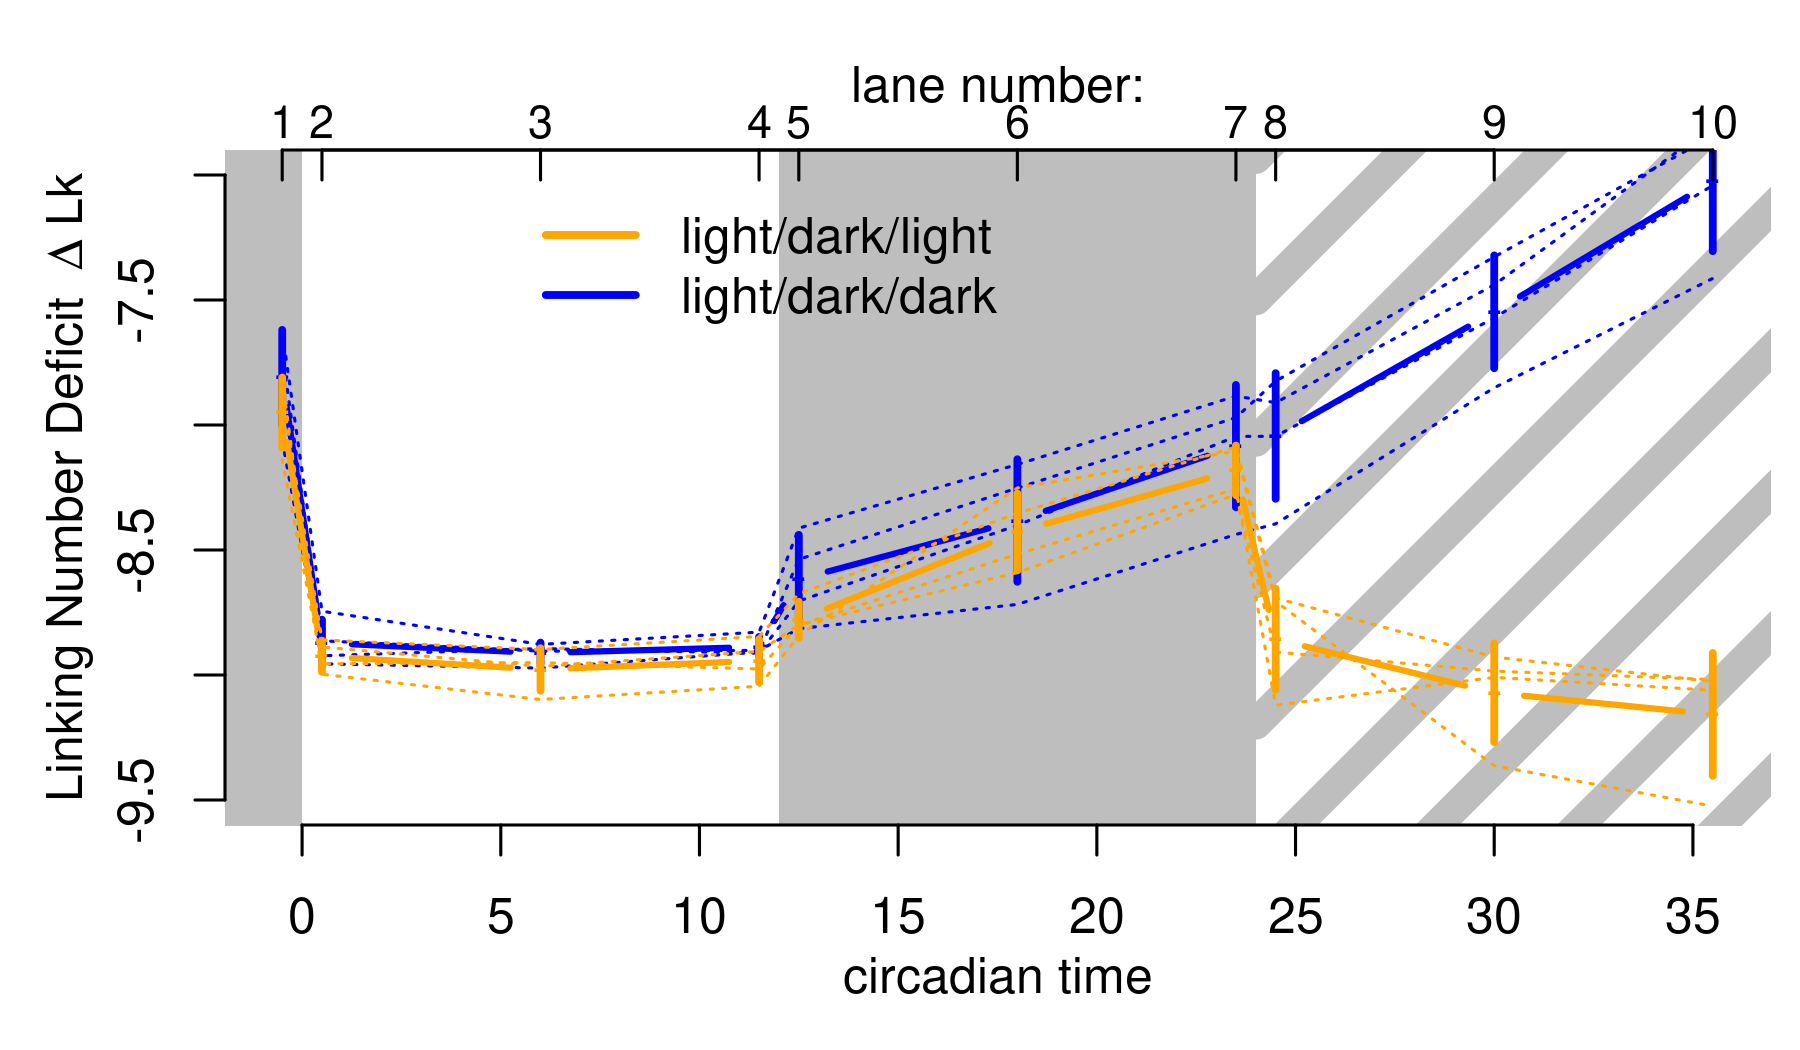
\includegraphics[width=\textwidth]{figures/diurnal/linkingNumbers.png}
  \end{minipage}
  
  \vspace{-.5cm}
  \textbf{B}\hspace{.48\textwidth}\textbf{D}
  \vspace{.2cm}
  
  \caption{\textbf{Diurnal Plasmid Supercoiling in
      \scyst{}}. \textbf{A \& B:} Southern blots with a probe for the
    pCA2.4\_M plasmid of \SI{1.2}{\percent} agarose gels supplemented
    with \SI{1}{\ugml} (A) or \SI{20}{\ugml} (B) CQ. The samples were
    extracted from two diurnal growth experiments and applied in the
    same order on both gels (see C). The central lane in (B) shows a
    pooled plasmid sample after treatment with the NcoI restriction
    enzyme which cuts only the pCA2.4\_M plasmid (one cut site) but
    not the similarly sized pCB2.4\_M. \textbf{C:} Example
    electropherogram of a single lane of topoisomers, extraced with
    ImageJ from a gel image and analyzed using peak detection routines
    to subtract a baseline (top, blue and green lines)) and calculate
    a mean linking number from topoisomer peak areas (bottom,
    $\dlk_\text{ref}=-8.24$).  \textbf{D:} Diurnal time-series of the
    average linking number deficits ($\Delta \overline{Lk}$) of the
    pCA2.4\_M plasmids, calculated from three replicates of agarose
    gels with \SI{20}{\ugml} (B) and the single replicate of the gel
    with \SI{1}{\ugml} (A).  The dotted thin lines are values from the
    4 different gels and the thick lines are their means and standard
    deviations.  Gray background indicates the dark phases. One
    culture (blue line, light/dark/dark) did not receive the final 12
    h of light and remained in the dark.  Note, that lower values
    indicate more negative supercoiling (higher $|\Delta
    \overline{Lk}|$). The absolute values of $\dlk$ are an estimate of
    $\dlkr$, based on the distance to the relaxed forms after topoI
    relaxation (not shown), and likely underestimates the real
    $|\dlkr|$.}
    \label{fig:blot} 
\end{figure}


\subsection{Gradual Plasmid Relaxation in Dark Phase, Quick Supercoiling in
  Light.}

To clarify the unresolved issue whether DNA supercoiling is higher
during the light or dark phases, we measured supercoiling levels of
endogenous plasmids of \textit{Synechocystis sp.} PCC6803 (``Moscow
strain'' PCC-M) \remove{and \textit{Synechococcus elongatus} PCC 7942}
during diurnal light/dark (\SI{12}{\hour}/\SI{12}{\hour}) conditions
and a prolonged dark phase (\SI{12}{\hour} light, followed by
h\SI{24}{\hour} darkness).  A large sample volume (\SI{25}{\mL}) was
required to obtain enough plasmids, and direct mixing of the sample
with an equal volume of pre-cooled (\SI{-20}{\celsius}) pure
undenatured ethanol was key to successful plasmid extraction. However,
the yield was still very low (\SIrange{0.5}{1}{\ug}, but incl. genomic
DNA), limiting the amount of gels that can be run from one sample.
%
Multiple sets of putative topoisomer bands were detected at all
sampled time points by agarose gel electrophoresis supplemented with
chloroquine at either \SI{1}{\ugml} or \SI{20}{\ugml}
(Fig. \ref{fig:blot}A, B). \scyst{} contains three short plasmids, two
at \SI{2.4}{kb} \cite{Yang1993b, Yang1994} and one at \SI{5.2}{kb}
\cite{Xu1997b}. Restriction analysis and Southern blots confirmed that
the most pronounced topoisomer bands were obtained for plasmid
pCA2.4\_M.
%
The migration distances on the gels were different between samples and
the relative differences reversed between the two CQ
concentrations. This change of relative migration speed indicates that
plasmids are still negatively supercoiled at the low, but positively
supercoiled at the high concentration. Plasmids which were originally
more relaxed migrate slower and faster at the low and high
concentrations, respectively.  \remove{Topo I relaxation time series
  of pooled samples from light and dark phases further confirmed that
  more relaxed plasmids migrate faster at the high CQ concentration
  (Fig. \ref{fig:topoi}A).}
%
Next, we quantified the agarose gels by generating electropherograms
of each lane in ImageJ. Baseline correction, peak detection and peak
area quantification were performed in R (Fig. \ref{fig:blot}C). For
each sample an average linking number deficit $\Delta \overline{Lk}$
was calculated and plotted as time series over the light/dark cycles
(Fig. \ref{fig:blot}D).  Plasmids were more negatively supercoiled
(lower $\Delta \overline{Lk}$) during light phases, and reached a
maximal level only \SI{30}{\minute} after transition to the light
phase. This level was maintained or only slightly increased throughout
the 12 h light phase.  During the dark phase the transition was
slower, and plasmids became progressively more relaxed during the 12
h, and relaxation continued at equal pace during an additional 12 h
dark phase.
%
The maximal linking number differences between light and dark phase
were only $\Delta \Delta \overline{Lk} \approx 1$, and $\Delta \Delta
\overline{Lk} \approx 2$ after the prolonged dark phase.

In summary, negative supercoiling of pCA is higher during the day,
with a quick increase directly after the onset of light, and lower
during the night; extended night relaxes plasmid even more. These
results are the exact opposite of the results reported by
\citet{Woelfle2007} for the endogenous plasmid of
\textit{Synechococcus elongatus} PCC 7942.  We believe that
\citet{Woelfle2007} had misinterpreted the relative topoisomer
mobilities, and the results are actually consistent between both
species. This conclusion is further supported by the silent reversal
of the interpretation of relative topoisomer mobilities by
\citet{Vijayan2009}.
  

\section{Conclusion}

Plasmid topoisomer analysis by intercalator-supplement relaxation
series and agarose gel electrophoresis is an old and elegant method.
However, the gels are difficult to interpret, and the effect of
intercalator concentrations must be checked for each plasmid and
conditions (gel and reaction buffers). Ideally, Keller's band counting
method should be applied to each newly analysed plasmid. The low
yields when extracting endogenous plasmids from cyanobacteria, the
time-intensive calibration routine, and non-standard electropherogram
analysis make it somewhat challenging to properly analyse \textit{in
  vivo} supercoiling in a given species.  Can these methods be
updated?

\citet{Mitchenall2018} reported separation of topoisomers of pBR322,
pUC19, and a 339 bp DNA minicircle on a commercial capillary gel
electrophoresis platform (Qiagen QIAxcel Advance System), where EtBr
is part of the gel delivered in a cartridge. The system is quite
sensitive and samples of \SI{100}{\ng} DNA sufficed. Moreover, the
range of separated topoisomers was broader than on agarose gels. This
would allow to use less runs with intercalator concentrations to
achieve full separation of \textit{in vivo} levels of supercoiling.
However, the intercalator type and concentration can not be
manipulated on this system. We recently succeeded to separate pUC19
topoisomers by adding comparatively large concentrations of CQ
($\cqgel=\SIrange{1}{3}{\milli\gram\per\liter}$) to the commercial
(and secret) gel delivered for the AATI Fragment Analyzer (now owned
by Agilent). But the results were not consistent between runs. Likely,
the undisclosed fluorescent nucleic acid marker has effects on DNA
supercoiling. More work and alternatives to the existing commercial
systems is required to establish topoisomer separation by capillary
gel electrophoresis as a standard procedure. This could potentially
greatly reduce the amount of sample required per run.

The analysis of electropherograms is also a limiting factor for many
laboratories. No standards or established tools exist on how to
calculate average linking number differences between
samples. Commerical gel image analysis software is not geared towards
this application. To this end \citet{Ziraldo2019} provide a plug-in
for the ImageJ image analysis software that could streamline the
analysis of agarose gels. Here, we also used ImageJ to extract
electropherograms from gel images, and peak detection routines from a
mass-spectrometry R package, \texttt{msProcess} (see Methods) which is
not maintained anymore, to calculate average linking numbers in R. A
novel R package, \texttt{bioanalyzeR}
(\url{https://github.com/jwfoley/bioanalyzeR}), allows to parse
electropherograms from data files exported by Agilent capillary
electrophoresis platforms (Bioanalyzer, TapeStation).
%
And finally, \citet{Vetcher2010} recently suggested a model that can
partially explain topoisomer mobility differences in agarose gels,
based on the writhe component $Wr$ of \dlk{}. Implementing such
theories in analysis tools could further support automatization.
Standardized and automated analysis tools for both, gel images and
capillary electrophoresis platforms could open this old and elegant
method for modern molecular biology laboratories.



\section*{Data Availability}
All gel images and electropherogramms are available on request. Our
chloroquine agarose protocols \TODO{will be made} available at
\url{protocols.io}. Custom and gel-specific R analysis scripts are
available on request.

\section*{Funding}
RM was funded by the \textit{Deutsche Forschungsgemeinschaft}, grants
AX~84/4-1, STA~850/30-1 and EXC-2048/1--project ID 390686111. 


\section{Materials and Methods}

\paragraph{pUC19 Plasmid Extraction.}
The vector DNA plasmid pUC19 (Roth: X911.1) was transferred into
\textit{Escherichia coli} DH5$\alpha$ via heat shock
transformation. DH5$\alpha$\_pUC19 was inoculated into LB medium and
grown overnight at \SI{37}{\celsius} and \SI{250}{rpm}. The preculture
was diluted 1:200 in fresh LB and grown for another \SI{3}{\hour}, and
harvested in exponential phase. The culture was centrifuged and pUC19
was isolated with ZymoPURE's Plasmid Maxiprep Kit. The isolated
plasmid was then purified (linear and open circular forms digested)
via T5 exonuclease (NEB: M0363) reaction and the NucleoSpin Gel and
PCR Clean-up kit (Machery-Nagel). The final plasmid DNA concentration
was determined with the Nanodrop (Thermo Scientific NanoDrop 2000c).
%
\paragraph{pUC19 Relaxation Series.}
The pUC19 plasmid extract was split and \SI{1}{\ug} samples were
incubated with 0--3000 \si{\ugml} chloroquine in \SI{24}{\uL} of the
CutSmart reaction buffer (50 mM potassium acetate, 20 mM Tris-acetate,
10 mM magnesium acetate, 100 \si{\ugml} BSA, pH 7.9) for \SI{15}{\min}
at \SI{37}{\celsius}. Then \SI{1}{\uL} (\SI{5}{U}) topoI (NEB: M0301)
was added and the samples incubated for another \SI{15}{\min} at the
same temperature. The reaction was stopped by incubation at
\SI{65}{\celsius} for \SI{20}{\min} and samples were purified with the
NucleoSpin Gel and PCR Clean-up kit (Machery-Nagel) to remove the
enzyme and the intercalator.

\paragraph{\scyst{} Strain and Culturing Conditions.}
Diurnal plasmid supercoiling time-series were established at
conditions and time-points identical to those used for the
transcriptome study in ref. \cite{Lehmann2013, Beck2014}.  The
glucose-tolerant and motile wild-type strain PCC-M of
\textit{Synechocystis} sp. PCC 6803 (obtained from S.  Shestakov,
Moscow State University, Russia), was grown photoautotrophically in
BG11-medium at \SI{30}{\celsius} under continuous illumination with
white light at \SI{80}{\photons} (Versatile environmental test
chamber; Sanyo) and with a continuous stream of air in two 
glass tube reactors with 800 mL culture volume.  The optical
density at 750 nm of the culture was monitored (Specord200 Plus;
Analytik Jena). Cultures where then entrained to 12 h/12 h light/dark
cycles for three consecutive days and diluted to $\OD{}\approx 0.5$
one day before sampling. Samples for plasmid analysis and \OD{} were
taken at the indicated timepoints for 1.5 days. One culture was
kept in dark for the last 12 h of sampling.

\paragraph{Plasmid Extraction from \scyst{} Cultures.}
\SI{25}{\mL} of cell culture were mixed with \SI{25}{\mL} of
pre-cooled undenatured 95\% ethanol (\SI{-80}{\celsius} and on dry ice
during sampling), in \SI{50}{\mL} centrifuge tubes and stored at
\SI{-80}{\celsius} until processing. After thawing on ice, the
supernatant was discarded after centrifugation for \SI{10}{\minute} at
\SI{4}{\celsius} and \SI{4000}{g}. The QIAprep Spin miniprep kit was
used according to manufacturer's instruction, except for additional
enzymatic steps during lysis. The cell pellet was resuspended in
\SI{250}{\micro\liter} Qiagen P1 solution and transferred to
\SI{1.5}{\mL} reaction tubes. Then \SI{50}{\micro\liter} lysozyme
solution (\SI{50}{\milli\gram\per\milli\liter}) was added, mixed, and
incubated for \SI{1}{\hour} at \SI{37}{\celsius}.  After the addition
of \SI{55}{\micro\liter} of \SI{20}{\percent} SDS and
\SI{3}{\micro\liter} of proteinase K
(\SI{20}{\milli\gram\per\milli\liter}), the reaction mixture was
incubated at \SI{37}{\celsius} for \SI{16}{\hour}.  Starting with the
alkaline lysis with the Qiagen P2 solution, all further steps (QIAprep
Spin Miniprep Kit) were carried out with amounts that were adjusted to
the initial volume. Next, the concentrations and quality (260/280,
230/280 ratio) was determined using the Nanodrop (Thermo Scientific
NanoDrop 2000c).  The PlasmidSafe enzyme mix (epicentre,
cat. no. E3101K) was used for removal of linear DNA according to the
manufacturer's protocol and incubated at \SI{37}{\celsius} for
\SI{30}{\minute} and purified with QIAprep spin columns using 5
volumes of the PB buffer. The final plasmid DNA concentration was
determined with the Nanodrop.


\paragraph{\scyst{} Plasmid Restriction Analyses.}
A pooled sample of plasmid extracts from \scyst{} was subjected to
rectriction by NcoI (Thermo Scientific: FD0573), which has a single
cut site in pCA2.4\_M but not in the similarly sized pCB2.4\_M.
\SI{1.5}{\uL} of FastDigest buffer and \SI{1}{\uL} of restriction
enzyme were added to \SI{12.5}{\uL} of plasmid samples. Reactions were
incubated for \SI{30}{\minute} at \SI{37}{\celsius} and stopped by
addition of \SI{3}{\uL} of 6x DNA loading dye with \SI{1}{\percent}
SDS and incubation at \SI{80}{\celsius} for \SI{15}{\minute}. The
resulting \SI{18}{\uL} were loaded directly onto the agaorse gels

\remove{To test plasmid relaxation by topoisomerase I pooled samples
  from light and dark phases were split and for each reaction
  \SI{10}{\uL} of plasmid extracts were mixed with \SI{5}{\uL} 3x
  reaction buffer (150 mM Tris, 150 mM KCl, 30 mM MgCl2 , 1.5 mM DTT,
  0.3 mM EDTA, \SI{90}{\ugml} BSA) with or without 1 U of TopoI
  (Invitrogen, Cat. no. 38042-024). The reactions were incubated at
  \SI{37}{\celsius} and stopped after the indicated times by addition
  of \SI{3}{\uL} of 6x DNA loading dye with \SI{1}{\percent} SDS at
  \SI{80}{\celsius} for \SI{15}{\minute}. The resulting \SI{18}{\uL}
  were loaded onto the agarose gel (Fig. \ref{fig:diurnalcq}E).}

\paragraph{Chloroquine Agarose Gel Electrophoresis.}
Agarose gels with different concentrations of chloroquine diphosphate
(CQ) were used to determine the relative migration speed of
supercoiled topoisomers. 1.2\% agarose gels in 0.5x TBE (5.4 g/L Tris
base, 2.75 g/L boric acid, 4 mL/L of 0.5 M EDTA (pH 8.0), pH 8.3).
were prepared by heating to boiling. After cooling (hand-warm) CQ was
added to the indicated final concentration from a stock solution
(\SI{10}{\milli\gram\per\milli\liter}) and the mixture poured into the
gel chamber. The running buffer was 0.5x TBE buffer with the same CQ
concentration as the gel. For each sample, \SI{250}{\ng}
(\textit{E. coli}/pUC19) or \SI{1}{\ug} (\scyst{}) of plasmid DNA were
mixed with loading dye and filled up to \SI{30}{\uL} with water.  Gels
were run for \SIrange{16}{24}{\hour} at \SI{40}{\volt}
(\SI{1.8}{\volt\per\cm}) in a Peqlab gel chamber, covered in foil to
protect from light. Gels were then washed two times for
\SI{30}{\minute} in \SI{250}{\mL} 0.5x TBE buffer to remove the CQ,
and stained with \SI{25}{\uL} Sybr Gold in \SI{225}{\mL} 0.5x TBE
buffer for \SIrange{3}{24}{\hour} and imaged on a BioRad Imaging
System (ChemiDoc MP). Washing and staining were also performed
light-protected.

\paragraph{Southern Blots of Agarose Gels.}

Probes for Southern blots were generated by colony PCR using the
primers in Table \ref{tab:blot} and the PCR programm: 3 min,
\SI{95}{\celsius}; 35x(\SI{95}{\celsius} 30s, \SI{50}{\celsius} 30s,
\SI{72}{\celsius} 1 min); \SI{72}{\celsius} 5 min.  The products were
isolated by cutting the band from an agarose gel and clean-up with the
NucleoSpin Extract II kit (Macherey-Nagel).  Labelled DNA was
generated using the same PCR program with the DIG Easy Hyb (Roche,
1603558) mix, according to manufacturer's instruction.
%
Southern blots were generated using the CDP-Star kit with slight
modifications as follows.  Gels were blotted onto a nitrocellulose
membrane using a vacuum blotter \remove{model?} (\SI{90}{\min} with
\SIrange{5}{7}{mm Hg}, in 10x SSC buffer). The membrane was
pre-hybridized for \SI{1}{\hour} at \SI{50}{\celsius}.  The probes
were denatured (\SI{95}{\celsius}, \SI{15}{\min}) and cooled on ice,
then transfered to the blot and hybridized over night at
\SI{50}{\celsius}. The membran was washed 2x \SI{5}{\min} mit 2x SSC,
0.1 \% SDS at \SI{50}{\celsius}, then with 2x 15 min mit 0.1x SSC und
0.1 \% SDS at \SI{65}{\celsius}, and cross-linked with UV light
\remove{model} for \SI{10}{\min}. All further steps were performed
according to the CDP-Star manual and blots were imaged on a
  BioRad Imaging System (ChemiDoc MP).

%Ich vermute, dass die Gele mit Dem Vakuum-Blotter geblottet wurden (mein Standard-Protokoll sagt, dass 90 min bei 5-7 mm Hg Unterdruck mit 10x SSC-Puffer geblottet wird). Danach wird die Membran zweimal mit 2x SSC-Puffer gewaschen und dann 5-10 min mit UV gecrosslinkt. Der Rest müsste so passen.




\begin{table}[ht!]
  \begin{tabular}{c|c|l}
    Plasmid & Direction & Sequence \\
    \hline
    pCA2.4\_M &forward & ACAGGGGTAAATGAGTGCCG\\ % grep-confirmed
    &reverse & GCAAGCAGTCCTCCACAAGA  % grep-confirmed, revcomp
  \end{tabular}
  \caption{\textbf{Southern Blot Probes: Primer Sequences.}}
  \label{tab:blot}
\end{table}


\paragraph{Analysis of Gel Electropherograms.}
Electropherograms were extracted in ImageJ for each lane and analyzed
in R, using LOESS smoothing and peak detection functions from the
\texttt{msProcess} R package (version 1.0.7)
(\url{https://cran.r-project.org/web/packages/msProcess/}). A baseline
was determined in two steps using the \texttt{msSmoothLoess} function
(Fig. \ref{fig:blot}C, top panel).  The first step used the full
signal and served to determine the coarse positions of peaks.  The
final baseline was then calculated from the signal after removal of
peak values. This baseline was subtracted from the total signal to
detect peaks (bands) with the \texttt{msPeakSimple} function from
\texttt{msProcess} and calculate peak areas.  For the total RNA
analysis, the baseline signal stems from mRNA and rRNA degradation
fragments, and was used to calculate ratios of rRNA peak areas to the
``baseline'' area.

\paragraph{Calculation of $\Delta Lk$.}
For the diurnal time series we quantified relative linking number
deficits (Fig. \ref{fig:blot}C, bottom panel) by analysis of
topoisomer peak areas.  Peaks were assigned consecutive
integral linking number values $\Delta Lk$ with an estimated offset of
a reference peak from the relaxed form with $Lk=0$. The areas under
the peaks $A_{\Delta Lk}$ were calculated and the average linking
number deficit of a sample was then determined as the center of mass
\begin{equation}
  \label{eq:dlk}
  \Delta \overline{Lk} = \sum{(\Delta Lk \cdot
    A_{\Delta Lk})}/\sum{A_{\Delta Lk}}
\end{equation}
of all topoisomer bands.

Note, that the true $\Delta Lk$ of bands from the relaxed plasmid was
not determined, eg. by Keller's band counting method
\cite{Keller1975b}.  The calculated $\Delta Lk$ values refer to an
assignment of a reference band that was present in all lanes to
$\Delta Lk=-8$, and this can be considered a maximal estimate of the
true $\Delta Lk$ based on the distance of topoisomer and relaxed DNA
bands in a topoI relaxation experiment (not shown).

\bibliographystyle{plainnat} %abbrvnat}%unsrt}
\setlength{\bibsep}{0.0pt}
\begin{spacing}{0.9}
  %% SWITCH between global and local/git bibtex file
  %% and use `bibexport -o cqgels.bib cqgels.aux` to update local
  % citations for goi.tex
  %\bibliography{/home/raim/ref/tata}
  \bibliography{cqgels}
\end{spacing}



\end{document}
